
%
\section{The signed core of a budgeted signed-binomial system}\label{sec:core}

% gloss: finely connected
This section proves Theorem~\ref{thm:core} for budgeted signed-binomial
systems (Definition~\ref{def:system}). If the feasible rational set is
bounded, two feasible rational points are finely connected, that is,
joined at every positive tolerance by sequences of feasible rational
points, exactly when their signed cores agree. This theorem is the engine of
Theorems~\ref{thm:boundary}(i), \ref{thm:fixed-profile}
and~\ref{thm:directed} and of Corollary~\ref{cor:algebraic}.

% ---------------------------------------------------------------------------
\subsection{Fine connectivity}\label{sec:fine-connectivity}

Fine Connectivity (Section~\ref{sec:binomial}) is the algebraic counterpart
of fixed-profile Fine Reachability in Section~\ref{sec:problem}. Its
vertices are feasible rational coordinate vectors, and its step bound uses
their sup norm. Section~\ref{sec:tractable} proves the transfer for
single-word tests. Fix a budgeted signed-binomial system on a finite
set~$J$ (Definition~\ref{def:system}). Recall that $\FQ$ is its feasible
rational set, and write $\FR$ for its real feasible set, which is closed.
Points $x,x'\in\FQ$ are \defterm{finely connected} if, for each rational
$\varepsilon>0$, feasible rational points join $x$ to $x'$ by sup-norm
steps below~$\varepsilon$. Fine connectivity is an equivalence relation,
since a sequence may be empty, reversed, or concatenated with another at
the same tolerance.

The example after Theorem~\ref{thm:core} shows that the signed-core
characterization can fail without boundedness of $\FQ$. Boundedness holds whenever every
coordinate lies in some budget, as in the Markov model.

% ---------------------------------------------------------------------------
\subsection{Restriction and the least support}\label{sec:restriction}

The classification compares what survives peeling, so we first show that
the survivor is well defined, although the active tests change from one
support to the next. We use the signed supports, the matrices
$\Delta_S$ of active tests, weight vectors, peeling steps $S\to T$ and
signed cores of Definition~\ref{def:system}. Lemma~\ref{lem:restriction}(c)
shows that the core $\core(S)$, the least support that $S$ peels to,
exists.

\begin{lemma}[Realization and restriction]\label{lem:restriction}
Fix a budgeted signed-binomial system on~$J$.
\begin{enumerate}
\item[(a)] Let $x\in\FQ$ have support~$S$, and let $S\to T$ be a peeling
step with weight vector~$\eta$. Put $x_j(t)=x_jt^{\eta_j}$ for $j\in S$ and
$x_j(t)=0$ otherwise, with $t^0=1$. Then $x(t)$ is feasible for
$0\le t\le1$, the point $x(0)$ has support~$T$ and agrees with $x$ on~$T$,
and $x$ and $x(0)$ are finely connected.
\item[(b)] If $S\to T$ and $U\subseteq S$, then $U\to U\cap T$. Hence, if
$S$ peels to~$T$, then $U$ peels to $U\cap T$.
\item[(c)] Every support $S$ has a unique least support $\core(S)$ that it
peels to, and every support that $S$ peels to has the same core. Two
supports have equal cores exactly when they peel to a common support, and
their common core lies in every such support.
\end{enumerate}
\end{lemma}

Lemma~\ref{lem:restriction} is proved in Appendix~\ref{app:core-proofs};
for~(c), a support of least cardinality that $S$ peels to lies, by~(b), in
every support that $S$ peels to. Restriction is what makes the core well
defined. Newman's lemma~\cite{newman} is the classical antecedent for such
uniqueness; here restriction proves it directly.

An \defterm{irreducible support} equals its own core, so no peeling step
reduces it. In the sign example, $\{y,z\}$ is irreducible. The P-hardness
proof of Section~\ref{sec:p-hardness} uses irreducible supports.

\begin{lemma}[The core is the greatest irreducible support]\label{lem:irreducible}
For every support~$S$, the core $\core(S)$ is irreducible and contains
every irreducible subset of~$S$, whether or not that subset is the support
of a feasible point. Hence $\core(S)$ is the greatest irreducible subset
of~$S$ and the union of all of them.
\end{lemma}

\begin{proof}
The core is irreducible, since $S$ peels to it and so it has the core
of~$S$ by Lemma~\ref{lem:restriction}(c). Let $F\subseteq S$ be
irreducible, and put $C=\core(S)$. By Lemma~\ref{lem:restriction}(b), $F$
peels to $F\cap C$, so $F=\core(F)\subseteq F\cap C$, and $F\subseteq C$.
\end{proof}

Figure~\ref{fig:peeling} runs this calculus on the staged example of
Section~\ref{sec:question}. Its coordinates are the eigenvalues $x,y,z$ of
the labels $\mathsf x,\mathsf y,\mathsf z$; in this and later examples,
letters name coordinates and points are written as tuples.
Its eigenvalue constraints are those of Section~\ref{sec:binomial}, and
the figure shows $x,y,z$. Starting from a
feasible point, each side of an active equation gains a power of~$t$. For
$0<t<1$, the equation stays satisfied exactly when the two exponents agree.
These balances form $\Delta_S\eta=0$.

On the starting support $S=\{x,y,z\}$, the probe equation $xy=xz$ and the
calibration $z=1/4$ are both active. The reversal equations impose no
additional conditions on the weights. The weights must therefore satisfy
\[
  \eta_y-\eta_z=0,\qquad \eta_z=0 .
\]
These equations allow $\eta_x=1$ and $\eta_y=\eta_z=0$, so a first peeling
step gives $\{x,y,z\}\to\{y,z\}$. They also force $\eta_y=0$, so no single
step reaches $\{z\}$.

Once $x=0$, the word test is still held and still passes. Its probe
equation is inactive because both monomials vanish. On $S=\{y,z\}$ only
\[
  \eta_z=0
\]
remains, so a second step gives $\{y,z\}\to\{z\}$ whatever the sign
of~$y$. The source $(1/4,1/4,1/4)$ takes two steps and the target
$(0,-1/4,1/4)$ one, and both reach the signed core $z$ alone, with
positive sign.

Recomputing the active tests is essential. A rule that keeps the starting
support's balance equations at every later support forces $\eta_y=0$ on
$\{y,z\}$. Each endpoint then keeps its own sign at~$y$, wrongly ruling out
the revision of Section~\ref{sec:question} (the dashed stubs in
Figure~\ref{fig:peeling}).

\begin{figure}[t]
  \centering
  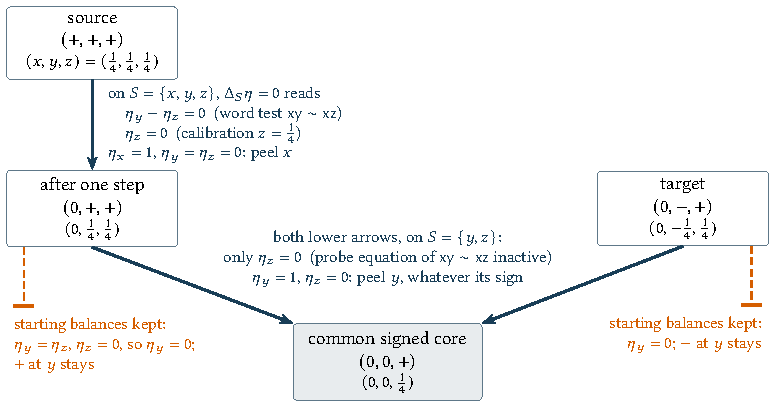
\includegraphics{figures/fig2-peeling.pdf}
  \Description{A flow diagram of signed supports in the coordinate order (x, y, z). The source, with signs (+, +, +) at the point (1/4, 1/4, 1/4), has an arrow to the node after one step, with signs (0, +, +) at (0, 1/4, 1/4); the arrow is labelled with the weight equations on the full support, eta_y - eta_z = 0 from the word test and eta_z = 0 from the calibration, solved by eta_x = 1, eta_y = eta_z = 0, which peels x. The node after one step and the target, with signs (0, -, +) at (0, -1/4, 1/4), both have arrows to the common signed core (0, 0, +) at (0, 0, 1/4). These arrows are labelled: on the support {y, z} only eta_z = 0 remains, because the probe equation of the word test is inactive, and eta_y = 1, eta_z = 0 peels y whatever its sign. Dashed stubs from the intermediate node and the target show what happens if the starting balances are kept. They force eta_y = 0, so the intermediate node retains positive y, the target retains negative y, and the two do not reach a common signed core.}
  \caption{Peeling the staged example of Section~\ref{sec:question}. Nodes
  are signed supports in the coordinate order $(x,y,z)$, each with a point
  that has it; arrow labels give the weight equations $\Delta_S\eta=0$ of
  the tests active on the current support~$S$. Recomputing them after each
  step leads the source (two steps) and the target (one step) to a common
  signed core. After the source's first step, the probe equation of
  $\mathsf{xy}\sim\mathsf{xz}$ is inactive. The dashed stubs keep the balance
  equations from the source support for both reductions. These force
  $\eta_y=0$ on $\{y,z\}$, leaving no common signed support to peel to.}\label{fig:peeling}
\end{figure}

% ---------------------------------------------------------------------------
\subsection{Computing the core}\label{sec:computing-core}

The core is computed by linear programming over recomputed supports. At
a support~$S$, a step removing $j\in S$ exists exactly when
$\Delta_S\eta=0$, $\eta\ge0$, $\eta_j\ge1$ has a rational solution, since
clearing denominators gives integer weights. Each round sums one solution
for each such~$j$, removing all removable coordinates at once, and
then recomputes the active tests. Every round but the last removes a
coordinate. The last can stop at a nonempty support, which has no proper
step and is therefore the core by Lemma~\ref{lem:restriction}(c). No
connectivity computation is needed, and Section~\ref{sec:algorithm} bounds
the cost. For a prescribed survivor set $T\subseteq S$, add $\eta_j=0$ on
$T$ and $\eta_j\ge1$ on $S\setminus T$ to $\Delta_S\eta=0$. This rational
feasibility test is equivalent to the existence of the peeling step
$S\to T$ after clearing denominators.

Related uses of linear programming occur in continuous Petri
nets and exponential families. Fraca and
Haddad's Algorithm~2~\cite{fracahaddad} alternates linear programming for
maximal state-equation support with forward and reverse firing-set
restrictions. For exponential families, Csiszár and
Matúš~\cite{csiszarmatus} characterize the variation closure of canonically
convex families using accessible faces. Geyer~\cite{geyer} uses repeated
linear programming in a method that identifies a limiting conditional model
via a generic direction of recession.

% ---------------------------------------------------------------------------
\subsection{Limits and exact interpolation}\label{sec:limits}

Necessity in Theorem~\ref{thm:core} must exclude sequences with ever finer
steps that pass between signed supports near a common limit point, which
can be irrational. A \defterm{real chart} is the set of points of $\FR$
with a given signed support, and a \defterm{rational chart} the set of
points of $\FQ$ with it.

\begin{lemma}[A chart limit gives a peeling step]\label{lem:limit}
Let points $x^{(k)}\in\RR^J$ satisfy every test of the system and share one
signed support~$\sigma$ with support~$S$, and let $x^{(k)}\to x^*\in\RR^J$.
Then $S\to\supp x^*$ is a peeling step, $x^*$ has the signs of $\sigma$ on
$\supp x^*$, and $\SC(x^*)=\SC(x^{(k)})$.
\end{lemma}

The proof, in Appendix~\ref{app:core-proofs}, takes logarithms on~$S$ and
keeps every test active on~$S$, including tests whose monomials vanish
at~$x^*$. %
Subtracting the bounded correction given by a fixed linear right inverse
produces a kernel vector on the vanishing coordinates. Negating this vector,
approximating in the rational kernel, clearing denominators and extending
by zero on the surviving coordinates yields a weight vector positive
exactly on $S\setminus\supp x^*$. No budget is used. The lemma can also be derived from Tevelev's criterion for
closures of subvarieties of a complex torus~\cite[Lemma~2.2]{tevelev}.
Sufficiency needs the opposite move.

\begin{lemma}[Rational interpolation]\label{lem:interpolation}
Any two points $x,x'\in\FQ$ with the same signed support are finely
connected through feasible rational points with that signed support.
\end{lemma}

The proof, also in Appendix~\ref{app:core-proofs}, samples the log-affine curve $\xi_j(t)=\sgn(x_j)|x_j|^{1-t}|x'_j|^{t}$ through the prime
factorizations of the endpoint ratios $|x'_j|/|x_j|$. Their exponent
vectors lie in the kernel of $\Delta_S$ and vanish on unchanged
coordinates. So the samples satisfy every test exactly, and tight budgets
on unchanged coordinates stay exact.

% ---------------------------------------------------------------------------
\subsection{The classification}\label{sec:classification}

The next lemma, proved in Appendix~\ref{app:core-proofs} and reused in
Section~\ref{sec:timing}, ties sequences with steps below every tolerance
to the connected components of a compact closure.

% seq{}uences: {} breaks the small-caps Qu ligature, which text extraction drops.
\begin{lemma}[Small-step seq{}uences in a compact closure]\label{lem:compact-chain}
Let $Y$ be a dense subset of a compact metric space~$Z$, and let
$h,h'\in Y$. %
The points $h$ and $h'$ lie in the same connected component of~$Z$ if and
only if, for every $\varepsilon>0$, there is a finite sequence in~$Y$ from
$h$ to~$h'$ whose consecutive distances are below~$\varepsilon$.
\end{lemma}

\begin{theorem}[Signed-core classification]\label{thm:core}
Let $J$ be finite. Fix finitely many tests $x^a=c\,x^b$ with
$a,b\in\NN^J$ and $c\in\QQ$, and finitely many $\ell^1$ budgets
$\sum_{j\in J_\beta}|x_j|\le\kappa_\beta$ with rational~$\kappa_\beta$.
Suppose the set $\FQ$ of feasible rational points is bounded. Then
$x,x'\in\FQ$ are finely connected if and only if $\SC(x)=\SC(x')$.
\end{theorem}

\begin{proof}
For sufficiency, iterating Lemma~\ref{lem:restriction}(a) along a peeling
from $\supp x$ to its core finely connects $x$ to a feasible rational
point $\hat x$ with support $\core(\supp x)$ that agrees with $x$ there.
Obtain $\hat x'$ from $x'$ in the same way. Equal signed cores give $\hat x$
and $\hat x'$ the same signed support, so Lemma~\ref{lem:interpolation}
joins them, and reversing the sequence from $x'$ completes the
sufficiency proof.

For necessity, let $\sigma$ range over the finitely many signed supports
of points of~$\FQ$, and let $K_\sigma$ be the closure of the rational chart
of~$\sigma$. Each $K_\sigma$ is compact by rational boundedness. If $K_\sigma$ and
$K_\tau$ meet at~$x^*$, Lemma~\ref{lem:limit} gives both charts the signed
core of~$x^*$. The unions of the sets $K_\sigma$ grouped by signed core
therefore form a finite family of pairwise disjoint compact sets. If at
least two classes occur, take $d>0$ to be the minimum of their pairwise
distances. Every feasible rational point lies in its own class union, so
no sequence with steps below $d$ changes class.
\end{proof}

Thus fine connectivity depends only on the support that survives iterated
peeling and on the signs there, not on magnitudes. The staged example's
endpoint eigenvalue vectors have equal signed cores, so they are finely
connected by Theorem~\ref{thm:core}. In the sign example, the probe
equation $y^2=z^2$ gives $2\eta_y=2\eta_z$, and the calibration gives
$\eta_z=0$. Thus $\{y,z\}$ is irreducible, and the different signs at $y$
give different signed cores. The two eigenvalue vectors are therefore not
finely connected.

Boundedness cannot be dropped. For $xy^2=1$ with no budgets, the balance
$\eta_x+2\eta_y=0$ forces zero weights, so both coordinates survive, and
the endpoints $(1,1)$ and $(1,-1)$ have different signed cores. Yet they
are finely connected: sample the rational points $(t^2,\pm1/t)$ finely
from $t=1$ to $t=n$ on each branch, and cross the gap $2/n<\varepsilon$
between the branches at $t=n$.

\begin{remark}[Components of the rational closure]\label{rem:closure}
Under the hypotheses of Theorem~\ref{thm:core}, the closure
$K=\overline{\FQ}$ is compact, and by Lemma~\ref{lem:compact-chain} points
of $\FQ$ are finely connected exactly when they lie in one component
of~$K$. Every component of $K$ meets~$\FQ$, although density alone would
not show this. Indeed, each point of $K$ lies in the closure of one of the
finitely many rational charts, each rational chart lies in one component
by Lemmas~\ref{lem:interpolation} and~\ref{lem:compact-chain}, and
components are closed. So the components of $K$ are labeled by the signed
cores of points of~$\FQ$. In the terms of Akin and
Wiseman~\cite[Section~3]{akinwiseman}, fine connectivity is the chain
relation of the identity map of $\FQ$ with the sup metric.
\end{remark}

Three objects must be kept apart: the real feasible set $\FR$, whose
components Corollary~\ref{cor:real} classifies; the closure $K$, which can
be strictly smaller; and finite rational sequences, which need no
continuous rational path. For $y^2=2x^2$ with $|x|+|y|\le1$, $K$ is the
origin and $\FR$ is two crossing segments. Under rational boundedness the
real and rational verdicts agree on rational endpoints in this class
(Corollary~\ref{cor:real}); Section~\ref{sec:real-rational} gives
instances with one word-against-pair test where they differ.

Three examples bound the theorem. For $xy=1$ with $|x|+|y|\le3$, the
balance $\eta_x+\eta_y=0$ forces zero weights, so two signed cores
survive, $(+,+)$ and $(-,-)$. The core can be empty even when no weight
vector is positive on the whole support. For $xy=x$ with $|x|+|y|\le2$,
the only proper one-step peel from full support removes~$x$. On $\{y\}$
the row is inactive, so $y$ then peels. Every feasible point has empty
core. Finally, the spherical section of $z_0z_2=z_1^2$ has two components,
while its budgeted affine cone has one signed core, so the theorem is not a
special case of Soprunova and Sottile's component
count~\cite[Theorem~2.4(2)]{soprunovasottile}.

Geometrically, on a fixed support~$S$, consider the damping-factor set
$\{e^{-\eta}:\eta\in\RR_{\ge0}^S,\ \Delta_S\eta=0\}$. With
$d_j=e^{-\eta_j}$, each balance becomes $d^a=d^b$, equivalently two
binomial inequalities on $(0,1]^S$, and the closure of this positive
solution set is a toric cube~\cite[Lemma~1 and Theorems~1--2]{toriccubes}.
Vanishing monomials can make some of these inequalities
vacuous~\cite[Example~3]{toriccubes}.

% ---------------------------------------------------------------------------
\subsection{Real components}\label{sec:real-components}

Over $\RR$ the same signed cores classify the components of the binomial
equations and budgets, with no boundedness at all.

% gloss: real component
\begin{corollary}[Real components]\label{cor:real}
Fix a budgeted signed-binomial system on a finite set~$J$, read over~$\RR$,
and let $\FR$ be its real feasible set, with no boundedness assumed. For
$x,x'\in\FR$ the following are equivalent: (i)~$x$ and $x'$ lie in one
connected component of~$\FR$; (ii)~a continuous path in $\FR$ joins them;
(iii)~$\SC(x)=\SC(x')$. If $\FQ$ is bounded, then for $x,x'\in\FQ$ these
conditions are also equivalent to fine connectivity.
\end{corollary}

\begin{proof}
A path lies in one component, so (ii) implies~(i). For (i)~implies~(iii),
consider the finitely many nonempty real charts. Every finite
limit of a real chart has the same signed core by Lemma~\ref{lem:limit}.
Each core class and its complement are therefore finite unions of chart
closures, so each class is relatively clopen. A connected set thus lies in
one class. For (iii)~implies~(ii), the monomial-curve calculation in the
proof of Lemma~\ref{lem:restriction}(a) applies to real feasible points:
the equations persist and every budget weakly decreases. Peeling $x$ and
$x'$ gives points $\hat x,\hat x'$ with the same signed support. The
log-affine interpolation from the proof of Lemma~\ref{lem:interpolation}
preserves the equations between these real points, and
$|\xi_j(t)|\le(1-t)|\hat x_j|+t|\hat x'_j|$ preserves the budgets.
Concatenating these paths (with the second peeling path reversed) proves~(ii).
The last claim follows from Theorem~\ref{thm:core}.
\end{proof}

Rational boundedness serves only the agreement, and the signed cores
occurring over $\RR$ and $\QQ$ can differ: $x^2=2$ with $|x|\le2$ has two
real components and no rational point. The classification is for binomial
equations: with $y=x^2$, $z=y$ and the affine trinomial $y+z=1$, the real
feasible set is the two points $(\pm1/\sqrt2,1/2,1/2)$, while the binomial
tests alone give both the empty core.

% gloss: P-complete
% gloss: PSPACE-hard
Section~\ref{sec:real-ncl} shows that deciding whether two supplied
feasible rational endpoints lie in the same real path component is
P-complete for binary-encoded budgeted signed-binomial systems under
deterministic log-space many-one reductions. Allowing a growing number of
scalar equations $x_j+y_j=1$ gives PSPACE-completeness under
polynomial-time many-one reductions.
